\documentclass[border=4pt,12pt]{standalone}
% House style for redrawn exam diagrams (diagram-v4: 0.4pt lines, filled -latex arrows, fine dashes; stipple and hatching drawn as real dots/lines (no PDF/SVG patterns, so they render in every browser and at any scale); transparent background). Every figure \input's this.
\usepackage{amsmath,amssymb}
\usepackage{txfonts}
\usepackage{pdfrender,xcolor}
% \halo{text}: label on shading. The shading stops just around each letter's outline (a thin knock-out that follows the
% glyphs, like the papers' typesetting), never a box. Owner: "I don't want a box around the text".
\newcommand{\halo}[1]{\leavevmode\rlap{\pdfrender{TextRenderingMode=2,LineWidth=2.2pt,LineJoinStyle=1,StrokeColor=white,FillColor=white}#1}#1}
\usepackage{tikz,pgfplots}
\pgfplotsset{compat=1.18}
\usetikzlibrary{arrows.meta,calc,angles,quotes,patterns,patterns.meta,intersections,positioning,decorations.markings,shapes.geometric}
% Stipple and hatching are drawn as actual dots / lines clipped to the region (path picture), NOT as pattern fills:
% SVG <pattern> fills vanish or blur when browsers scale the image, so the owner could not see the shading.
% Each dot is a 0.72pt square (keeps SVGs small; reads as a dot at print size). Dots sit on one global staggered grid, so neighbouring regions line up.
\makeatletter
\newdimen\ex@x \newdimen\ex@y \newdimen\ex@xa \newdimen\ex@ya \newdimen\ex@xb \newdimen\ex@yb \newcount\ex@row
\def\exam@stipplecolor{black!75}\def\exam@dotr{0.42pt}\def\exam@dotgap{2.5}
\def\ex@rowdots{\ifdim\ex@x<\ex@xb \pgfpathrectangle{\pgfqpoint{\dimexpr\ex@x-0.36pt\relax}{\dimexpr\ex@y-0.36pt\relax}}{\pgfqpoint{0.72pt}{0.72pt}}\advance\ex@x by \exam@dotgap pt\relax\expandafter\ex@rowdots\fi}
\def\exam@stipple{%
  \pgftransformreset% dots are sized in real points even inside scaled pictures
  \pgfpointanchor{path picture bounding box}{south west}\ex@xa=\pgf@x \ex@ya=\pgf@y
  \pgfpointanchor{path picture bounding box}{north east}\ex@xb=\pgf@x \ex@yb=\pgf@y
  \pgfsetfillcolor{\exam@stipplecolor}\pgfmathsetmacro\ex@h{\exam@dotgap/2}%
  \pgfmathtruncatemacro\ex@r{floor(\ex@ya/\ex@h)-1}\ex@row=\ex@r\relax
  \ex@y=\ex@r\dimexpr\ex@h pt\relax
  \loop\ifdim\ex@y<\ex@yb
    \pgfmathtruncatemacro\ex@c{floor(\ex@xa/\exam@dotgap)-1}\ex@x=\ex@c\dimexpr\exam@dotgap pt\relax
    \ifodd\ex@row \advance\ex@x by \ex@h pt\fi
    \ex@rowdots
    \advance\ex@y by \ex@h pt \advance\ex@row by 1
    \ifnum\numexpr\ex@row-(\ex@row/4)*4\relax=0 \pgfusepath{fill}\fi% flush every 4 rows: bounded TeX memory, few clip copies in the SVG
  \repeat\pgfusepath{fill}}
\newdimen\ex@d
\def\exam@hatch#1{% #1 = 1 for /, -1 for \ ; lines 45 degrees, 3pt apart
  \pgftransformreset
  \pgfpointanchor{path picture bounding box}{south west}\ex@xa=\pgf@x \ex@ya=\pgf@y
  \pgfpointanchor{path picture bounding box}{north east}\ex@xb=\pgf@x \ex@yb=\pgf@y
  \ex@d=\dimexpr\ex@yb-\ex@ya\relax \ex@x=\dimexpr\ex@xa-\ex@d\relax
  \loop\ifdim\ex@x<\ex@xb
    \ifnum#1>0 \pgfpathmoveto{\pgfqpoint{\ex@x}{\ex@ya}}\pgfpathlineto{\pgfqpoint{\dimexpr\ex@x+\ex@d\relax}{\ex@yb}}%
    \else \pgfpathmoveto{\pgfqpoint{\ex@x}{\ex@yb}}\pgfpathlineto{\pgfqpoint{\dimexpr\ex@x+\ex@d\relax}{\ex@ya}}\fi
    \advance\ex@x by 4.24pt
  \repeat
  \pgfsetlinewidth{0.4pt}\pgfsetstrokecolor{black}\pgfusepath{stroke}}
\def\examstipple{\exam@stipple}\def\examhatch{\exam@hatch}\def\examsetstipplecolor#1{\def\exam@stipplecolor{#1}}\def\examsetdotgap#1{\def\exam@dotgap{#1}}
\makeatother
% (legacy pattern kept for old files)
% staggered stipple like the NESA papers' dotted shading
\pgfdeclarepatternformonly{exam stipple}{\pgfpointorigin}{\pgfqpoint{2.2pt}{2.2pt}}{\pgfqpoint{2.2pt}{2.2pt}}{%
  \pgfpathcircle{\pgfqpoint{0.55pt}{0.55pt}}{0.42pt}\pgfpathcircle{\pgfqpoint{1.65pt}{1.65pt}}{0.42pt}\pgfusepath{fill}}
\tikzset{
  every picture/.style={line width=0.6pt, >={Latex[length=2mm,width=1.3mm]}},
  curve/.style={line width=0.6pt},
  open arrow/.style={-{Latex[length=2mm,width=1.3mm]}},  % owner: filled -latex heads everywhere, no open chevrons
  aux/.style={dash pattern=on 2pt off 1.5pt, line width=0.6pt},
  shade/.code={\def\exA{#1}\def\exB{none}\ifx\exA\exB\else\pgfkeysalso{fill=black!18}\fi},
  shade/.default=on,
  shade dots/.style={fill=none, path picture={\examstipple}},
  stipple color/.code={\examsetstipplecolor{#1}},
  stipple gap/.code={\examsetdotgap{#1}},
  shade dense dots/.style={fill=none, stipple gap=1.6, path picture={\examstipple}},
  shade hatch/.style={fill=none, path picture={\examhatch{1}}},
  shade hatch reverse/.style={fill=none, path picture={\examhatch{-1}}},
  shade solid/.style={fill=black},
  pt/.style={circle, fill, inner sep=1.1pt},
  open pt/.style={circle, draw, fill=white, inner sep=1.1pt},
}
\pgfplotsset{
  exam axes/.style={axis lines=middle, axis line style={->}, xlabel={$x$}, ylabel={$y$},
    xlabel style={anchor=west}, ylabel style={anchor=south}, tick label style={font=\small},
    every axis plot/.append style={line width=0.6pt, black}, samples=200, clip=false,
    enlargelimits=false, axis on top},
}

\begin{document}
% Redrawn from the RTA road-map poster (checker 25 Nov: "recreate the diagram"; it was kept as the scanned crop).
% Kept: the two highways, the towns and both distance scales from Sydney. Left out: the poster border, its slogans and logo.
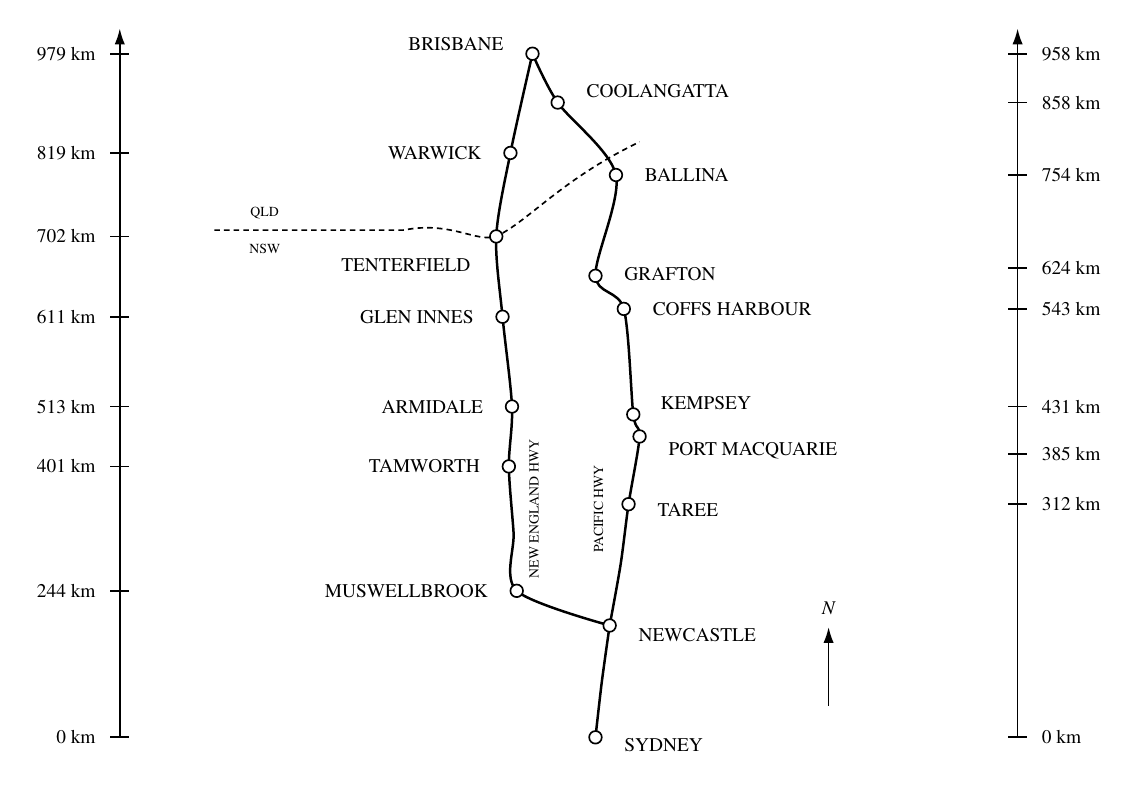
\begin{tikzpicture}[x=0.02cm,y=-0.02cm,every node/.style={font=\scriptsize}]
\coordinate (Syd) at (272,590); \coordinate (New) at (281,519);
\coordinate (Mus) at (222,497); \coordinate (Tam) at (217,418); \coordinate (Arm) at (219,380);
\coordinate (Gle) at (213,323); \coordinate (Ten) at (209,272); \coordinate (War) at (218,219);
\coordinate (Bri) at (232,156);
\coordinate (Tar) at (293,442); \coordinate (Por) at (300,399); \coordinate (Kem) at (296,385);
\coordinate (Cof) at (290,318); \coordinate (Gra) at (272,297); \coordinate (Bal) at (285,233);
\coordinate (Coo) at (248,187);
% state border (dashed) and labels
\draw[aux] (30,268) -- (150,268) .. controls (180,262) and (196,276) .. (209,272) .. controls (230,262) and (250,236) .. (300,212);
\node[font=\tiny] at (62,257) {QLD};
\node[font=\tiny] at (62,280) {NSW};
% roads
\draw[line width=0.9pt] plot[smooth,tension=0.5] coordinates {(Syd) (276,555) (New)};
\draw[line width=0.9pt] plot[smooth,tension=0.5] coordinates {(New) (Mus) (220,460) (Tam) (Arm) (Gle) (Ten) (War) (Bri)};
\draw[line width=0.9pt] plot[smooth,tension=0.5] coordinates {(New) (288,480) (Tar) (Por) (Kem) (Cof) (Gra) (Bal) (Coo) (Bri)};
\node[font=\tiny,rotate=90] at (233,445) {NEW ENGLAND HWY};
\node[font=\tiny,rotate=90] at (274,445) {PACIFIC HWY};
\foreach \p in {Syd,New,Mus,Tam,Arm,Gle,Ten,War,Bri,Tar,Por,Kem,Cof,Gra,Bal,Coo} \filldraw[fill=white] (\p) circle (4);
% town names: New England towns to the left, Pacific towns to the right
\node[anchor=east] at (210,497) {MUSWELLBROOK};
\node[anchor=east] at (205,418) {TAMWORTH};
\node[anchor=east] at (207,380) {ARMIDALE};
\node[anchor=east] at (201,323) {GLEN INNES};
\node[anchor=east] at (199,290) {TENTERFIELD};
\node[anchor=east] at (206,219) {WARWICK};
\node[anchor=east] at (220,150) {BRISBANE};
\node[anchor=west] at (293,525) {NEWCASTLE};
\node[anchor=west] at (284,595) {SYDNEY};
\node[anchor=west] at (305,446) {TAREE};
\node[anchor=west] at (312,408) {PORT MACQUARIE};
\node[anchor=west] at (307,378) {KEMPSEY};
\node[anchor=west] at (302,318) {COFFS HARBOUR};
\node[anchor=west] at (284,296) {GRAFTON};
\node[anchor=west] at (297,233) {BALLINA};
\node[anchor=west] at (260,180) {COOLANGATTA};
% distance scales from Sydney (km): New England Highway on the left, Pacific Highway on the right
\draw[->] (-30,590) -- (-30,140);
\foreach \y/\d in {497/244,418/401,380/513,323/611,272/702,219/819,156/979}
  {\draw (-36,\y) -- (-24,\y); \node[anchor=east] at (-39,\y) {$\d$ km};}
\draw[->] (540,590) -- (540,140);
\foreach \y/\d in {442/312,410/385,380/431,318/543,292/624,233/754,187/858,156/958}
  {\draw (534,\y) -- (546,\y); \node[anchor=west] at (549,\y) {$\d$ km};}
\draw (-36,590) -- (-24,590); \node[anchor=east] at (-39,590) {$0$ km};
\draw (534,590) -- (546,590); \node[anchor=west] at (549,590) {$0$ km};
% north arrow
\draw[->] (420,570) -- (420,520); \node at (420,508) {$N$};
\end{tikzpicture}
\end{document}
